\documentclass[12pt]{article}
\usepackage{geometry}
\usepackage{dcolumn}
\usepackage{booktabs}
\usepackage{pdflscape}
\usepackage{graphicx}
\usepackage{placeins}
\usepackage{dcolumn}
\usepackage{booktabs}
\linespread{1.5}

\begin{document}
\title{Connected Stocks}
\author{S.Morteza Aghajanzadeh}
\maketitle

We have connected stocks through their common blockholder. By controlling for style and sector similarity, and many other pair characteristics Is the degree of shared ownership forecasts cross-sectional variation in return correlation?

\section{Measuring Common Ownership}


At each week, we measure common ownership as the total value of stock held by the F common blockholder of the two stocks, scaled by the total market
capitalization of the two stocks, and label this variable $ FCAP_{ij,t} $.
Thus, $ FCAP_{ij,t} = \frac{\sum_{f = 1}^{F} (S^f_{i,t}P_{i,t}+S^f_{j,t}P_{j,t})}{S_{i,t}P{i,t} + S_{j,t}P{j,t}} $ where $ S^f_{i,t} $ is the number of shares held by blockholder $ f $ at time t trading at price $ P_{i,t} $ with total shares outstanding of $ S_{i,t} $, and similarly for stock j. We define common blockholder as those blockholder that held both stocks i and j in their portfolios at the end of quarter t. For each cross section, we calculate the
normalized (to have zero mean and unit standard deviation) rank-transformed  $ FCAP_{ij,t} $, which we denote as $ FCAPF_{ij,t} $.
we summarize our data in figure \ref{f1} and \ref{f2}.


\begin{figure}[htbp]
\centering
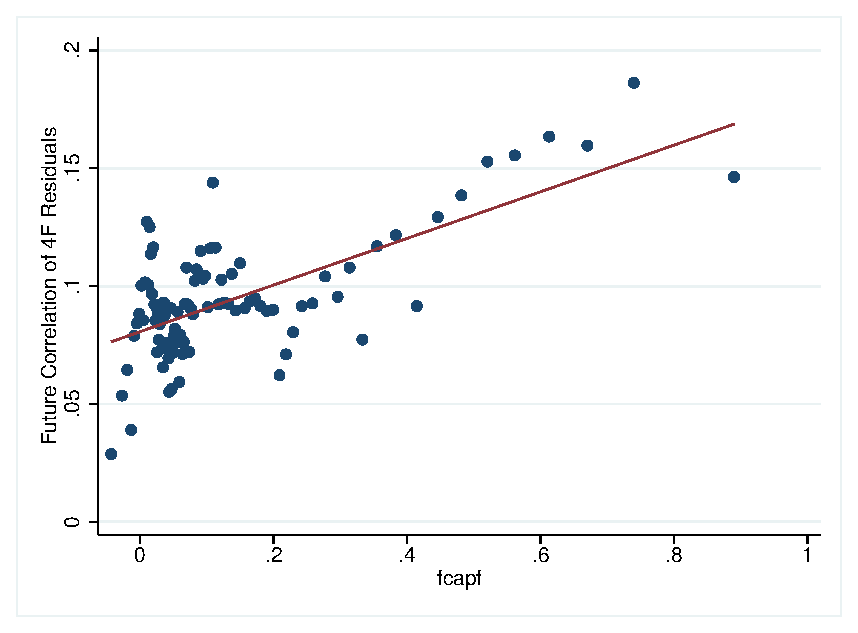
\includegraphics[width = 0.7\columnwidth ]{mygraph2.eps}
\caption{Future Correlation via FCAPF}
\label{f1}
\end{figure}

\begin{figure}[htbp]
\centering
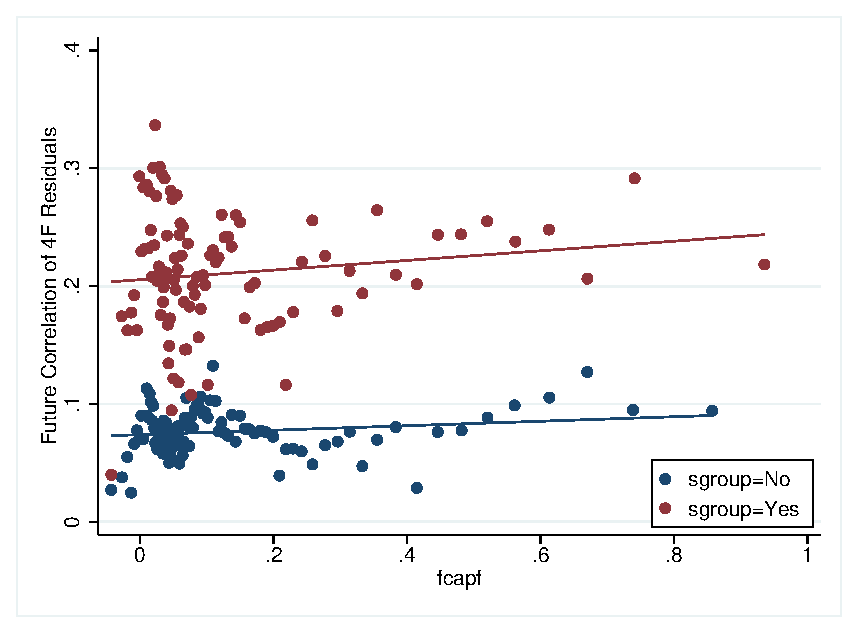
\includegraphics[width = 0.7\columnwidth ]{mygraph.eps}
\caption{Future Correlation via FCAPF grouped by same industry}
\label{f2}
\end{figure}


\FloatBarrier
\section{Regression}

We estimate cross-sectional regressions forecasting the within-week realized
correlation $ \rho_{ij,t+1} $ of each stock pair’s weekly with $ FCAPF_{ij,t} $ and a host of pair characteristics that we use as controls:
\begin{equation}
\rho_{ij,t+1} = a + b_f \times FCAPF_{ij,t} + \sum_{k = 1}^{n } CONTROL_{ij,t,k} + \varepsilon_{ij,t+1}
\label{e1}
\end{equation}

\subsection{Dependent Variable}
we use difference types of correlations for estimating via regression. we define future correlation by lag of $ l $ by this formula $ \rho_{fl} =  \rho_{t+l} $.

\subsection{Control Variables}
we control for similarity in characteristics
directly. To measure this similarity each week, we first calculate stock’s market ratio ,which means ratio of stocks' market capitalization to total market capitalization , SIZE1 and SIZE2 (where we label the
larger stock in the pair as the first stock). After that, we define SAMESIZE that is the normalized absolute difference in market ratio of two stocks.
we define dummy variable SGROUP to check if two stocks belong to same industry or not.

Further more, we use past correlation of stocks. we define past correlation by lag of $ l $ by this formula $ \rho_{fl} =  \rho_{t-l} $.

\newgeometry{top=5mm, bottom=5mm,left = 5mm,right = 5 mm}

%\toprule
%                    &\multicolumn{3}{c}{Cluster(t)}                                   &\multicolumn{3}{c}{Cluster(id)}                                  \\\cmidrule(lr){2-4}\cmidrule(lr){5-7}
%                    &\multicolumn{1}{c}{$ \rho4 $}&\multicolumn{1}{c}{$  \rho4_f $}&\multicolumn{1}{c}{$  \rho4_{f2} $}&\multicolumn{1}{c}{$  \rho4 $}&\multicolumn{1}{c}{$  \rho4_f $}&\multicolumn{1}{c}{$  \rho4_{f2} $}\\
%\midrule



\begin{landscape}
\begin{table}
\centering
\input{example.tex}
\end{table}

\end{landscape}
\restoregeometry


\begin{table}
\centering
\lr{
\def\sym#1{\ifmmode^{#1}\else\(^{#1}\)\fi}
\begin{tabular}{l*{6}{c}}
\hline\hline
            &\multicolumn{1}{c}{(1)}&\multicolumn{1}{c}{(2)}&\multicolumn{1}{c}{(3)}&\multicolumn{1}{c}{(4)}&\multicolumn{1}{c}{(5)}&\multicolumn{1}{c}{(6)}\\
            &\multicolumn{1}{c}{$ \rho4_f $}&\multicolumn{1}{c}{$ \rho4_f $}&\multicolumn{1}{c}{$ \rho4_f $}&\multicolumn{1}{c}{$ \rho4_f $}&\multicolumn{1}{c}{$ \rho4_f $}&\multicolumn{1}{c}{$ \rho4_f $}\\
\hline
fcapf       &       0.132\sym{***}&       0.125\sym{***}&      0.0460\sym{***}&      0.0380\sym{***}&      0.0381\sym{**} &      0.0360\sym{**} \\
            &     (10.70)         &      (9.43)         &      (4.42)         &      (3.62)         &      (3.47)         &      (3.22)         \\
[1em]
$ \rho4 $        &                     &      0.0741\sym{***}&                     &                     &      0.0685\sym{***}&      0.0650\sym{***}\\
            &                     &      (5.98)         &                     &                     &      (5.54)         &      (5.37)         \\
[1em]
sgroup      &                     &                     &       0.151\sym{***}&       0.144\sym{***}&       0.135\sym{***}&       0.126\sym{***}\\
            &                     &                     &     (16.52)         &     (16.00)         &     (14.56)         &     (14.26)         \\
[1em]
samesize    &                     &                     &                     &      0.0944\sym{***}&      0.0892\sym{***}&                     \\
            &                     &                     &                     &      (6.63)         &      (6.46)         &                     \\
[1em]
size1       &                     &                     &                     &                     &                     &     0.00526         \\
            &                     &                     &                     &                     &                     &      (0.24)         \\
[1em]
size2       &                     &                     &                     &                     &                     &       0.645\sym{***}\\
            &                     &                     &                     &                     &                     &      (6.82)         \\
[1em]
size1*size2&                     &                     &                     &                     &                     &      -0.684\sym{***}\\
            &                     &                     &                     &                     &                     &     (-6.66)         \\
[1em]
\_cons      &      0.0763\sym{***}&      0.0702\sym{***}&      0.0685\sym{***}&      0.0981\sym{***}&      0.0913\sym{***}&      0.0237         \\
            &      (7.27)         &      (7.26)         &      (6.57)         &      (7.53)         &      (7.61)         &      (1.23)         \\
\hline
\(N\)       &      326500         &      311086         &      326500         &      326500         &      311086         &      311086         \\
\hline\hline
\multicolumn{7}{l}{\footnotesize \textit{t} statistics in parentheses}\\
\multicolumn{7}{l}{\footnotesize \sym{*} \(p<0.05\), \sym{**} \(p<0.01\), \sym{***} \(p<0.001\)}\\
\end{tabular}
}

\end{table}



\FloatBarrier
\section{Panel Regression}
At this section we estimate equation \ref{e1} by using fixed effect regression via panel data.

\begin{table}[htbp]
\centering
{
\def\sym#1{\ifmmode^{#1}\else\(^{#1}\)\fi}
\begin{tabular}{l*{5}{c}}
\hline\hline
            &\multicolumn{1}{c}{(1)}&\multicolumn{1}{c}{(2)}&\multicolumn{1}{c}{(3)}&\multicolumn{1}{c}{(4)}&\multicolumn{1}{c}{(5)}\\
            &\multicolumn{1}{c}{$ \rho $}&\multicolumn{1}{c}{$ \rho_f $}&\multicolumn{1}{c}{$ \rho_{f2} $}&\multicolumn{1}{c}{$  \rho_{f3} $}&\multicolumn{1}{c}{$ \rho_{f5} $}\\
\hline
fcapf       &     -0.0139\sym{*}  &     -0.0160\sym{*}  &     -0.0181\sym{**} &     -0.0200\sym{**} &     -0.0184\sym{**} \\
            &     (-2.15)         &     (-2.44)         &     (-2.68)         &     (-2.92)         &     (-2.61)         \\
[1em]
pcorr\_6     &    -0.00128         &     -0.0190         &     -0.0137         &     -0.0123         &     -0.0128         \\
            &     (-0.13)         &     (-1.94)         &     (-1.38)         &     (-1.23)         &     (-1.26)         \\
[1em]
pcorr\_12    &     -0.0114         &     -0.0112         &     0.00440         &      0.0201\sym{*}  &      0.0110         \\
            &     (-1.18)         &     (-1.15)         &      (0.44)         &      (2.02)         &      (1.09)         \\
[1em]
\_cons      &       0.175\sym{***}&       0.180\sym{***}&       0.173\sym{***}&       0.169\sym{***}&       0.178\sym{***}\\
            &     (27.60)         &     (28.14)         &     (26.75)         &     (25.80)         &     (26.86)         \\
\hline
\(N\)       &       11076         &       10942         &       10644         &       10469         &       10081         \\
\hline\hline
\multicolumn{6}{l}{\footnotesize \textit{t} statistics in parentheses}\\
\multicolumn{6}{l}{\footnotesize \sym{*} \(p<0.05\), \sym{**} \(p<0.01\), \sym{***} \(p<0.001\)}\\
\end{tabular}
}

\end{table}

\begin{table}
\centering
{
\def\sym#1{\ifmmode^{#1}\else\(^{#1}\)\fi}
\begin{tabular}{l*{4}{c}}
\hline\hline
            &\multicolumn{1}{c}{(1)}&\multicolumn{1}{c}{(2)}&\multicolumn{1}{c}{(3)}&\multicolumn{1}{c}{(4)}\\
            &\multicolumn{1}{c}{$ \rho_{f3} $}&\multicolumn{1}{c}{$ \rho_{f3} $}&\multicolumn{1}{c}{$ \rho_{f3} $}&\multicolumn{1}{c}{$ \rho_{f3} $}\\
\hline
fcapf       &    -0.00601         &     -0.0200\sym{**} &    -0.00401         &     -0.0171\sym{*}  \\
            &     (-1.21)         &     (-2.92)         &     (-0.80)         &     (-2.48)         \\
[1em]
pcorr\_6     &                     &     -0.0123         &                     &     -0.0132         \\
            &                     &     (-1.23)         &                     &     (-1.32)         \\
[1em]
pcorr\_12    &                     &      0.0201\sym{*}  &                     &      0.0189         \\
            &                     &      (2.02)         &                     &      (1.90)         \\
[1em]
size1       &                     &                     &      -0.169         &     -0.0555         \\
            &                     &                     &     (-1.09)         &     (-0.29)         \\
[1em]
size2       &                     &                     &       4.493\sym{***}&       4.097\sym{***}\\
            &                     &                     &      (4.67)         &      (3.59)         \\
[1em]
size1\#size2&                     &                     &      -4.657\sym{*}  &      -4.596         \\
            &                     &                     &     (-2.18)         &     (-1.91)         \\
[1em]
\_cons      &       0.167\sym{***}&       0.169\sym{***}&       0.157\sym{***}&       0.158\sym{***}\\
            &     (35.88)         &     (25.80)         &     (28.89)         &     (20.83)         \\
\hline
\(N\)       &       18391         &       10469         &       18391         &       10469         \\
\hline\hline
\multicolumn{5}{l}{\footnotesize \textit{t} statistics in parentheses}\\
\multicolumn{5}{l}{\footnotesize \sym{*} \(p<0.05\), \sym{**} \(p<0.01\), \sym{***} \(p<0.001\)}\\
\end{tabular}
}

\end{table}

\end{document}